% !TEX TS-program = pdflatex
% !TEX encoding = UTF-8 Unicode

% This is a simple template for a LaTeX document using the "article" class.
% See "book", "report", "letter" for other types of document.

\documentclass[11pt]{article} % use larger type; default would be 10pt

\usepackage[utf8]{inputenc} % set input encoding (not needed with XeLaTeX)

%%% Examples of Article customizations
% These packages are optional, depending whether you want the features they provide.
% See the LaTeX Companion or other references for full information.

%%% PAGE DIMENSIONS
\usepackage{geometry} % to change the page dimensions
\geometry{a4paper} % or letterpaper (US) or a5paper or....
% \geometry{margin=2in} % for example, change the margins to 2 inches all round
% \geometry{landscape} % set up the page for landscape
%   read geometry.pdf for detailed page layout information

\usepackage{graphbox}
% \usepackage{graphicxbox}
\graphicspath{{img/}}
\usepackage{tabularx}
\usepackage{listings}
\usepackage{amsmath}

% \usepackage[parfill]{parskip} % Activate to begin paragraphs with an empty line rather than an indent

%%% PACKAGES
\usepackage{booktabs} % for much better looking tables
\usepackage{array} % for better arrays (eg matrices) in maths
\usepackage{paralist} % very flexible & customisable lists (eg. enumerate/itemize, etc.)
\usepackage{verbatim} % adds environment for commenting out blocks of text & for better verbatim
\usepackage{subfig} % make it possible to include more than one captioned figure/table in a single float
% These packages are all incorporated in the memoir class to one degree or another...

%%% HEADERS & FOOTERS
\usepackage{fancyhdr} % This should be set AFTER setting up the page geometry
\pagestyle{fancy} % options: empty , plain , fancy
\renewcommand{\headrulewidth}{0pt} % customise the layout...
\lhead{}\chead{}\rhead{}
\lfoot{}\cfoot{\thepage}\rfoot{}

%%% SECTION TITLE APPEARANCE
\usepackage{sectsty}
\allsectionsfont{\sffamily\mdseries\upshape} % (See the fntguide.pdf for font help)
% (This matches ConTeXt defaults)

%%% ToC (table of contents) APPEARANCE
\usepackage[nottoc,notlof,notlot]{tocbibind} % Put the bibliography in the ToC
\usepackage[titles,subfigure]{tocloft} % Alter the style of the Table of Contents
\renewcommand{\cftsecfont}{\rmfamily\mdseries\upshape}
\renewcommand{\cftsecpagefont}{\rmfamily\mdseries\upshape} % No bold!

%%% END Article customizations

\newcommand{\imgtex}{\begin{tabularx}{\textwidth}{@{}c@{ }X@{}}}

%%% The "real" document content comes below...

\title{Automated Redstone Manual}
\author{by CD4017BE}
\date{mod version: 4.2.2}

\begin{document}
 \maketitle
 \tableofcontents
 
 \section{About this manual}  
Ingame there already is basic information about the blocks and items available in their tooltips if you press SHIFT. So this manual contains the more detailed information about how things work in Automated Redstone as well as giving some examples. But crafting recipes are not available here, use the Just Enough Items (JEI) mod to view them ingame. It's also recommended to look up other Items to if they are mentioned in tooltips.

Most screenshots used here are edited to make them fit better into the document, so don't worry if your ingame should look a bit different. 

The information provided here refers to the mod version displayed above.

\section{Redstone Signals}
Minecraft represents the redstone output state (aka. redstone strength) of blocks by using 32-bit-integer numbers which theoretically allow redstone signal values up to $2.147.483.647$ as well as negative numbers. The components provided by Automated Redstone take advantage of this and can operate with pretty high numbers. Also \bf Redstone Cards \bf from the \bf OpenComputers \rm mod support full range so these mods can work together very well.

But most redstone components provided by minecraft itself and also most mods can only handle and emit values in range $0-15$. So expect that anything above or below is interpreted as only 15 or 0. The \bf Redstone Comparator \rm is the only component in vanilla minecraft that also works with values above 15.\\

To transmit these bigger numbers, the mod provides two new types or redstone wires that also have a few other advantages over "vanilla redstone":

Signals can be transported over (theoretically) unlimited distance and won't change their value (loose strength). Also these wires can be placed anywhere and don't need a solid surface.
To allow very compact wiring, wires laying next to each other can be disconnected by sneak-right-click. And for decoration you can cover them with solid blocks via right-click with the block in hand.

\subsection{Signals as binary numbers}
Signals in this mod are generally just an array of states (a.k.a. bits) that each can be either inactive or active. Signals with multiple bits can also be used to represet other types of data than just binary states, for example numbers:

Integer numbers are represented as $X = bit_0*2^0 + bit_1*2^1 + \dots + bit_N*2^N$ with $bit=0$ for inactive and $1$ for active states. This works almost the same way we represent our decimal numbers with the digits 0-9 ($X=digit_0*10^0 + digit_1*10^1 + \dots + digit_N*10^N$). So for example the number 42 represented as $4*10 + 2 * 1$ in decimal, is represented as $1*32 + 0*16 + 1*8 + 0*4 + 1*2 + 0*1$ (101010) in binary. Therefore in the same way you need at least two digits to represent the numbers 0-99 you need 4 bits to represent the numbers 0-15 in binary. Generally with $N$ bits you can represent numbers in range $0$ up to $2^N - 1$. \it This was probably not new to you if you already have experience with programming.\rm 

Some devices in this mod have settings called "external bit offset"($o$) and "signal size"($s$) which simply define the range of bits a redstone signal should be received or emitted on. When setting $o = 0, s = 32$ (default) the signal ($X$) will be always equal the the redstone strength ($R$). With an offset $o > 0$ the signal will start at a higher bit index and with a size $s < 32$ the signal is capped off after s bits. When using numbers this means $X= \frac{R}{2^o} \mod 2^s$ for received signals and $R = (X \mod 2^s) * 2^o$ for emitted signals.

When using the circuit you will probably often work with single bit states (only active or inactive). In this case use a signal size of 1 and if want to emit an active state as full redstone strength use an offset of 4 which will result in a strength of 16. When receiving signals of strength 15 (default for vanilla emitters) it doesn't matter whether you use 0,1,2 or 3 as offset but if it's a different strength and you don't want to worry about which bit has to be used, just move the signal through a Redstone Repeater (turns everything not 0 into 15).

\subsection{Solid Redstone Wire}
\bf Solid Redstone Wires \rm support signal values in range 0-255. They will receive redstone signals from their input connections (blue) and transmit them further to their output connections (green) with one tick delay. If one has multiple inputs it will choose the highest signal value for output. To control the signal transfer direction, these cables come in three variants:\\
\bf Input cables \rm will by default connect to neighboring (non replaceable) blocks in the world and receive signals from these. They will try to establish output connections to other cables if possible.\\
\bf Output cables \rm also connect to other blocks and will emit their signal to them. They will try to establish input connections to other cables.\\
\bf Transport cables \rm only connect to other cables and will establish their connections so that they transport signals from input to output cables. They also connect to some other devices in this mod on their own. If you already used the basic item/fluid transport pipes from \bf Inductive Automation \rm you will notice that the connection behavior is the same.\\
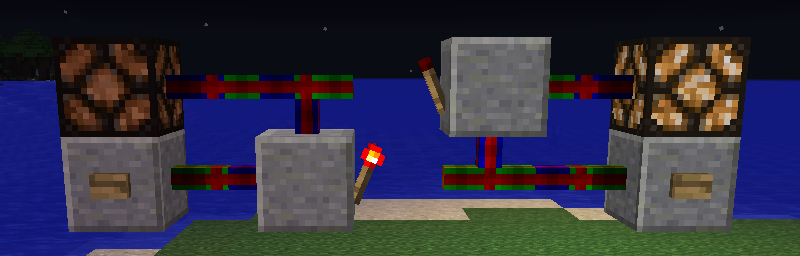
\includegraphics[width=\textwidth]{1_bit_pipes}\\

\subsection{32-bit Signal Wire}
\bf 32-bit Signal Wires \rm support full integer range and work a bit different:
Here you can set each side of each block individually to be either input(blue), output(green), both(cyan) or none(not connected), right-click with empty hand to cycle. The output signal for all outputs is calculated by combining all input signals on the whole connected wire system via bitwise OR operation.

It's recommended to not connect a wire to itself via input and output or two wires to each other via bidirectional connection because you would end up with self-sustaining redstone signals.

\section{Signal components}
\subsection{8-bit Lever}
The \bf 8-bit lever \rm provides redstone signals in range $000\dots255$. It has a front side with 8 red switches that binary encode the block's output signal. The upper row encodes 1 2 4 8 and the lower row 16 32 64 128. Each lever can be flipped by simple right click, down is off and up is on.

\subsection{Signal LED-display}
The \bf Signal LED-display \rm displays the redstone signal it is receiving. When right clicked it will open its GUI that allows detailed configuration about how to display:
Signal bit offset and signal size define which bits of the input signal should be used to encode the number. Leave them at 0 32 to use all bits, unless you are transmitting multiple separate numbers within one signal. Numbers can be displayed in either decimal (normal) or hexadecimal (base 16) mode using the format string or in binary mode as 8 lamps that are oriented the same like in the 8-bit Lever.
The two text fields on top and bottom are for description texts that will be shown above and below the number.
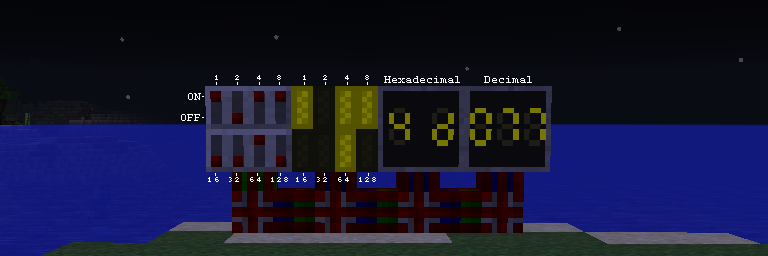
\includegraphics[width=\textwidth]{8_bit_io}\\

\newpage
\section{Sensors}
\bf Sensor Modules \rm are used to detect certain properties usually from the block they are linked to. To use them for redstone control mechanisms they can be put into a \bf Sensor Module Container \rm. When opening its GUI there are 6 slots (one for each block face) that can hold Sensor Modules:\\

\includegraphics[width = \textwidth]{sensor_gui}\\
The two numbers next to each slot define how the value ($X$) measured by the Sensor Module should be converted into the redstone signal ($R$) that is emited on its block face.\\
$R(X) = X*multiplier+offset$ While $X$, $multiplier$ and $offset$ are all floating point numbers, $R$ will be rounded down to the next full integer. So using the right multiplier and offset you can perform any linear transformation on the measurement value.

When giving the output to a Repeater, Redstone Torch or anything else that doesn't care about the actual strength, it's also possible to just use the transformation as comparator:\\
for $X\geq C$ use $multiplier=1$ and $offset=1-C$.\\
for $X\leq C$ use $multiplier=-1$ and $offset=1+C$.\\

\subsection{Item Sensor}
The \bf Item Sensor \rm counts the amount of matching items in the inventory of the blockface, it's linked to (some blocks have side dependent inventories). If the block has no inventory, it will instead use the items that would be dropped when harvested or items laying around in that spot.

The \bf Item Sensor \rm has a filter and will only count those items matching to it (or the amount of empty slots in the inventory if the filter is set to allow nothing). The filter can be edited via GUI on right-click in air.

\subsection{Fluid Sensor}
The \bf Fluid Sensor \rm counts the amount (mB) of matching fluids in tanks provided at the linked blockface. The linked block can also be a fluid block in the world, in this case the amount is usually the bucket volume of 1000mB.

The \bf  Fluid Sensor \rm has a filter and will only count those fluids matching to it (or the remaining tank capacity if the filter is set to allow nothing). The filter can be edited via GUI on right-click in air.

\subsection{Energy Sensor}
The \bf Energy Sensor \rm counts the amount of energy stored in its linked block in units of kJ (InductiveAutomation's energy unit). It also supports Blocks using the folowing energy types from other mods: RedstoneFlux (1RF = 0.1kJ), Tesla (like RF), IndustrialCraft (1EU = 0.4kJ). Keep in mind that these other energy types will be translated in to their equivalent kJ amount, so for example 250RF will be represented as 25kJ.

\subsection{Time Sensor}
The \bf Time Sensor \rm has 4 operating modes:\\

\includegraphics[align=c]{time_total} outputs the time difference in seconds between the current time (\& date) and the set starting date.\\

\includegraphics[align=c]{time_int} is like above but resets the starting date every time, the set interval is passed.\\

\includegraphics[align=c]{time_reset} outputs the time in seconds passed  since the last time, the linked blockface emitted redstone.\\

\includegraphics[align=c]{time_diff} outputs the time in seconds between the last two times, the linked blockface emitted redstone.\\
And you can choose one of the following timer types to be used for the measurement:\\
\bf Server Ticks \rm is based on the total amount of calculation cycles (ticks) the world has been simulated so far, where each tick represents $0.05s$. In case the server becomes unable to maintain its normal tickrate of 20 calculation cycles per second, the timer will slow down and stay synced with all other game processes.\\
\bf Ingame Time \rm behaves similar but is based on the ingame time and therefore in sync with daytime and moon phases (1 ingame day = 20min). So this timer will do jumps when players go sleeping or somebody uses time editing commands.\\
\bf System Time \rm is based on the internal clock of your computer or server and will always be in sync with real time, no matter how much the server was lagging or has been offline.\\

\newpage
\section{Integerated redstone circuits}
\imgtex

\includegraphics[align = t]{circuit} & The \bf Redstone Circuit \rm block allows you to put complicated redstone logic circuits into one single block, making them very compact and a bit cheaper in redstone cost. To define what the block should do you need to program it using the \bf Circuit Programmer \rm (explained later).\\
\end{tabularx}

\subsection{Creating \& using a circuit}
\imgtex

\includegraphics[align = t]{assembler} & Before the circuit can do anything or even be written with a program, you have to install components to it in the \bf Circuit Assembler\rm . There are four different types of components (IO-bits, storage bytes, logic gates and calculators), each required for certain functionality:\\
\end{tabularx}

\bf IO-bits \rm are required for communication with neighboring blocks, so you always need them. The amount depends on how many and how complex signals the circuit should receive or emit (explained with circuit GUI). Maximum amount is 192 (allowing full 32-bit signals on all 6 sides).

\bf Storage bytes \rm each provide a chunk of 8 bits which are required to store the result of logic gates and operators or externally received signals. Maximum is 32 byte (256 bit). 

\bf Logic Gates \rm and \bf Calculators \rm are required to install programs. You will be told how much of each is needed in \bf Circuit Programmer \rm when trying to store a program on a circuit.\\
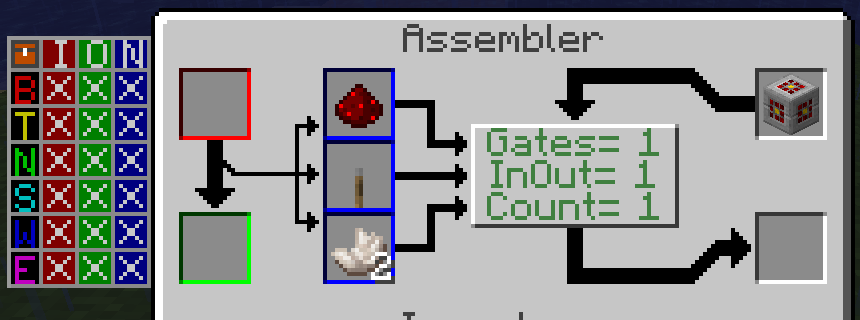
\includegraphics[width = \textwidth]{assembler_gui}\\
The circuit goes into the slot on the right and components are added by putting the required items in the 4 blue slots and pressing the '+' buttons. Circuits put into the red slot will get disassembled by outputting all contained component items back into the blue slots.\\

When the circuit is placed it has to be turned on and you have to define which block faces should be connected with which of the storage bits in its GUI:\\
\imgtex
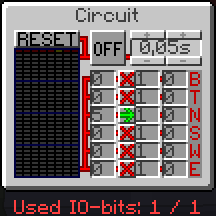
\includegraphics[align=t]{circuit_gui} & 
For each side there is a row of settings. The button defines whether the side is input, output or inactive and the numbers define where the signal should be put in or read from the storage, its size and its external strength-bit offset \it(for details see section 2.1)\rm . The dot grid on the left shows the current state of all storage bits, dark red are in inactive state, bright red active and the gray ones are unused (install more storage byte components to use them). When hovering over a side config row, all storage bits connected with that block face will show in yellow. Also you can set the time interval for processing cycles (+/- buttons), start or pause processing (ON/OFF) and set all storage bits back to inactive (RESET).
\end{tabularx}\\
Every time the tick interval you've set is passed, the circuit will perform the following processing cycle:

First all redstone signals received on the input sides are transfered into the storage bits they are connected to.

Next all the logic gates and operators from the stored program are recalculated and put their results on the storage bits they were defined on. This is done one by one in the same order as they were defined in the program. Note that if there is no program written on the circuit it will still run and just skip this part, meaning that the circuit won't be able to do much more than just move signals from one side to another.

Finally the output sides will read their new signal from the storage bits they are connected to and emit them to neighbor blocks (causing block updates if the signal changed).
\subsection{Programming}
Programming circuits works a bit different than usual computer programming languages. 
\imgtex 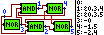
\includegraphics[align = t, scale = 2]{program_diagram} & The program basically defines a bunch of logic gates and operators and how they are wired together. This is an example schematic of a toggle latch with its source code on the right to demonstrate how the programming works. (node 0 is input and 4,5 are output)\end{tabularx} \\
Each line in the program represents one of the circuit's storage bits and defines how to calculate its (next) state. It usually starts with one character representing it's type and is directly (no whitespace) followed by its parameters which are separated by colons ',' (also no whitespace).

There are three types of parameters: \bf Bits \rm are written as the hexadecimal index number of the storage bit to use as input (its line number). For \bf Bytes \rm it's the '\#' character followed by the decimal index number of the storage byte that should be used to form the input number in binary out if its 8 bits. And \bf Constants \rm are just written as decimal number in range 0-255.

All currently available operation types are listed in this table: \\
\begin{tabularx}{\textwidth}{|c|c|l|X|} \hline
\bf Type & \bf Ch & \bf Parameters & \bf Function \\\hline
OR gate & $+$ & 0-15 bits & Active if any input active, otherwise inactive. \\\hline
NOR gate & $-$ & 0-15 bits & Inactive if any input active, otherwise active. \\\hline
AND gate & $\&$ & 0-15 bits & Inactive if any input inactive, otherwise active. \\\hline
NAND gate & $*$ & 0-15 bits & Active if any input inactive, otherwise inactive. \\\hline
XOR gate & $/$ & 0-15 bits & Active if uneven number of inputs active. \\\hline
XNOR gate & $\backslash$ & 0-15 bits & Active if even number of inputs active. \\\hline
$A < B$ & $<$ & byte/const A,B & Active if input number A smaller than B. \\\hline
$A \geq B$ & $>$ & byte/const A,B & Active if input number A not smaller than B. \\\hline
$A = B$ & $=$ & byte/const A,B & Active if input numbers A and B equal. \\\hline
$A \neq B$ & $\widetilde{}$ & byte/const A,B & Active if input numbers A and B not equal. \\\hline
Counter & $\$$ & S, A, R, B & Increases its count by constant A if bit S active and resets it to constant B if bit R active. \\\hline
Extension & $.$ & none & Used in lines following a counter to provide additional bits to store its binary count number. \\\hline
\end{tabularx}\\
\it There is also a short version of this as hovering tooltip in the Programmer GUI. \rm\\
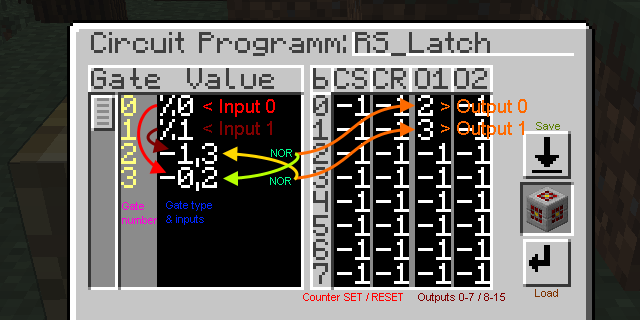
\includegraphics[width = \textwidth]{programmer_gui}\\
% TODO describe GUI navigation and code auto completion here
To put your settings onto a circuit, just give it a name in the line on top, put the circuit into the only available slot and click the save button. If everything is fine you should get a "Compiling successful" message and the tooltip of the circuit should show the program name you have set. If your gate definitions contain errors you get a message that tells "Compile error" with the line that was wrong. Otherwise if your circuit is missing gates, counter or outputs required to execute your settings you get a message that tells you what is missing.

To store your settings for later use you can also save it on a piece of paper and later load it into the programmer again by clicking the load button. If you don't need a circuit program anymore just put the item into the crafting grid to get the paper back.

\subsection{Example programms}
A \bf timer \rm that emits a 1 tick redstone signal every 150 ticks and resets if receiving a signal:
\begin{lstlisting}
Program:
0:		input signal
1: =#1,149	check if counter reached 149
2: +0,1		reset counter if it reached 149 or input active
3: -0		increase counter if input not active
8: $3,1,2,0	counter increases by 1 and resets to 0
9-F: .		8-bit counter
IO settings:
0, In, 1, 0	input signal
2, Out, 1, 4	output signal
\end{lstlisting}
A \bf clock \rm that displays time in minutes and seconds on two 8-bit Displays. It has a 'run' and a 'reset' input for control. (Circuit tick interval must be set to 0.05s):
\begin{lstlisting}
Program:
0:		run signal
1:		reset signal
2: =#1,19	check if 19 ticks have passed
3: =#2,59	check if 59 seconds have passed
4: &2,3		reset second counter after 59.95s
5: +1,4		or if receiving reset signal
6: +1,2		reset tick counter after 19 ticks or reset signal
8: $0,1,6,0	counting ticks
9-C: .		5-bit counter
10: $2,1,5,0	counting seconds
11-15: .	6-bit counter
18: $4,1,1,0	counting minutes
19-1F: .	8-bit counter
IO settings:
0, In, 1, 0	run
1, In, 1, 0	reset
10, Out, 6, 0	display seconds (6-bit)
18, Out, 8, 0	display minutes (8-bit)
\end{lstlisting}

\it there will be probably added more in the future \rm
%TODO add more programs here

\end{document}